\begin{figure}[H]
\centering
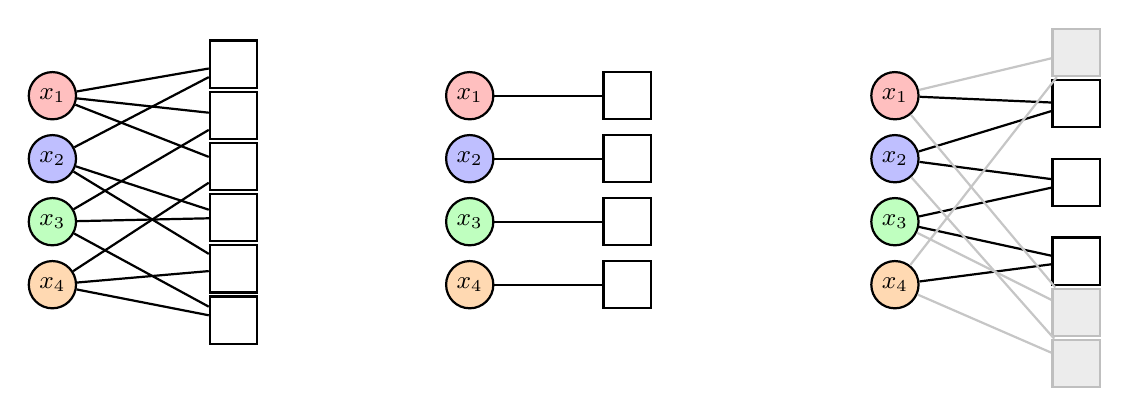
\begin{tikzpicture}[
    font=\small,
    % variable colors
    v1/.style={circle, draw, thick, fill=red!25,    minimum size=6mm, inner sep=0pt},
    v2/.style={circle, draw, thick, fill=blue!25,   minimum size=6mm, inner sep=0pt},
    v3/.style={circle, draw, thick, fill=green!25,  minimum size=6mm, inner sep=0pt},
    v4/.style={circle, draw, thick, fill=orange!30, minimum size=6mm, inner sep=0pt},
    fac/.style={rectangle, draw, thick, minimum width=6mm, minimum height=6mm, inner sep=0pt},
    facfaded/.style={rectangle, draw, thick, draw=gray!50, fill=gray!15,
        minimum width=6mm, minimum height=6mm, inner sep=0pt},
    edge/.style={draw, thick},
    faded/.style={draw, thick, gray!45},
]

% =========================================================
% Left panel: full dependency graph as 6 pairwise factors
% =========================================================
\begin{scope}[shift={(0,0)}]
% variables
\node[v1] (v1L) at (0,  1.2) {$x_1$};
\node[v2] (v2L) at (0,  0.4) {$x_2$};
\node[v3] (v3L) at (0, -0.4) {$x_3$};
\node[v4] (v4L) at (0, -1.2) {$x_4$};

% factors
\node[fac] (f12L) at (2.3,  1.60) {};
\node[fac] (f13L) at (2.3,  0.95) {};
\node[fac] (f14L) at (2.3,  0.30) {};
\node[fac] (f23L) at (2.3, -0.35) {};
\node[fac] (f24L) at (2.3, -1.00) {};
\node[fac] (f34L) at (2.3, -1.65) {};

% edges
\draw[edge] (v1L) -- (f12L);
\draw[edge] (v2L) -- (f12L);

\draw[edge] (v1L) -- (f13L);
\draw[edge] (v3L) -- (f13L);

\draw[edge] (v1L) -- (f14L);
\draw[edge] (v4L) -- (f14L);

\draw[edge] (v2L) -- (f23L);
\draw[edge] (v3L) -- (f23L);

\draw[edge] (v2L) -- (f24L);
\draw[edge] (v4L) -- (f24L);

\draw[edge] (v3L) -- (f34L);
\draw[edge] (v4L) -- (f34L);
\end{scope}

% =========================================================
% Middle panel: fully factorized (4 unary factors)
% =========================================================
\begin{scope}[shift={(5.3,0)}]
% variables
\node[v1] (v1M) at (0,  1.2) {$x_1$};
\node[v2] (v2M) at (0,  0.4) {$x_2$};
\node[v3] (v3M) at (0, -0.4) {$x_3$};
\node[v4] (v4M) at (0, -1.2) {$x_4$};

% unary factors
\node[fac] (f1M) at (2.0,  1.2) {};
\node[fac] (f2M) at (2.0,  0.4) {};
\node[fac] (f3M) at (2.0, -0.4) {};
\node[fac] (f4M) at (2.0, -1.2) {};

% edges
\draw[edge] (v1M) -- (f1M);
\draw[edge] (v2M) -- (f2M);
\draw[edge] (v3M) -- (f3M);
\draw[edge] (v4M) -- (f4M);
\end{scope}

% =========================================================
% Right panel: tree cover (3 kept pairwise factors, 3 discarded faded)
% =========================================================
\begin{scope}[shift={(10.7,0)}]
% variables
\node[v1] (v1R) at (0,  1.2) {$x_1$};
\node[v2] (v2R) at (0,  0.4) {$x_2$};
\node[v3] (v3R) at (0, -0.4) {$x_3$};
\node[v4] (v4R) at (0, -1.2) {$x_4$};

% retained tree factors
\node[fac]      (f12R) at (2.3,  1.10) {};
\node[fac]      (f23R) at (2.3,  0.10) {};
\node[fac]      (f34R) at (2.3, -0.90) {};

% discarded factors
\node[facfaded] (f14R) at (2.3,  1.75) {};
\node[facfaded] (f13R) at (2.3, -1.55) {};
\node[facfaded] (f24R) at (2.3, -2.20) {};

% retained edges
\draw[edge] (v1R) -- (f12R);
\draw[edge] (v2R) -- (f12R);

\draw[edge] (v2R) -- (f23R);
\draw[edge] (v3R) -- (f23R);

\draw[edge] (v3R) -- (f34R);
\draw[edge] (v4R) -- (f34R);

% discarded edges
\draw[faded] (v1R) -- (f14R);
\draw[faded] (v4R) -- (f14R);

\draw[faded] (v1R) -- (f13R);
\draw[faded] (v3R) -- (f13R);

\draw[faded] (v2R) -- (f24R);
\draw[faded] (v4R) -- (f24R);
\end{scope}

\end{tikzpicture}
\caption{Factor-graph representations induced by different posterior approximations. Left: the full dependency structure represented with one pairwise factor for each variable pair. Middle: a fully factorized approximation with unary factors only. Right: a tree-cover approximation retaining only the factors associated with the selected tree edges; faded factor nodes indicate discarded dependencies.}
\label{fig:chapter_5_controlled_graph_structure_dependencies}
\end{figure}